\subsection{在pdf中嵌入代码}在\LaTeX 中嵌入代码有多种方法。可以使用的包有:listings、minted、tcolorbox等方式。

\subsection{参考文献相关}
\paragraph{引入参考文件}引入参考文献时,可以使用.bib文件的方式引入参考文件。写好.bib文件后,需要按序执行以下四步完成引用:
\begin{enumerate}
	\item 先编译.tex文件。个人认为是编译.tex文件,为参考文献产生位置
	\item 编译.bib文件(一般使用bibtex),生成编译后的参考文献
	\item 再编译.tex文件,这时会将参考文献引入到.tex编译后的文件中(好像是.aux文件)。但这时在正文中可能不会正常显示
	\item 再次编译.tex文件即可得到引用正确、显示正确的pdf
\end{enumerate}

\subsection{数学符号}
\paragraph{数学字体}其中某些单元格的内容可能出错了,只需要把多余的字符去掉即可。
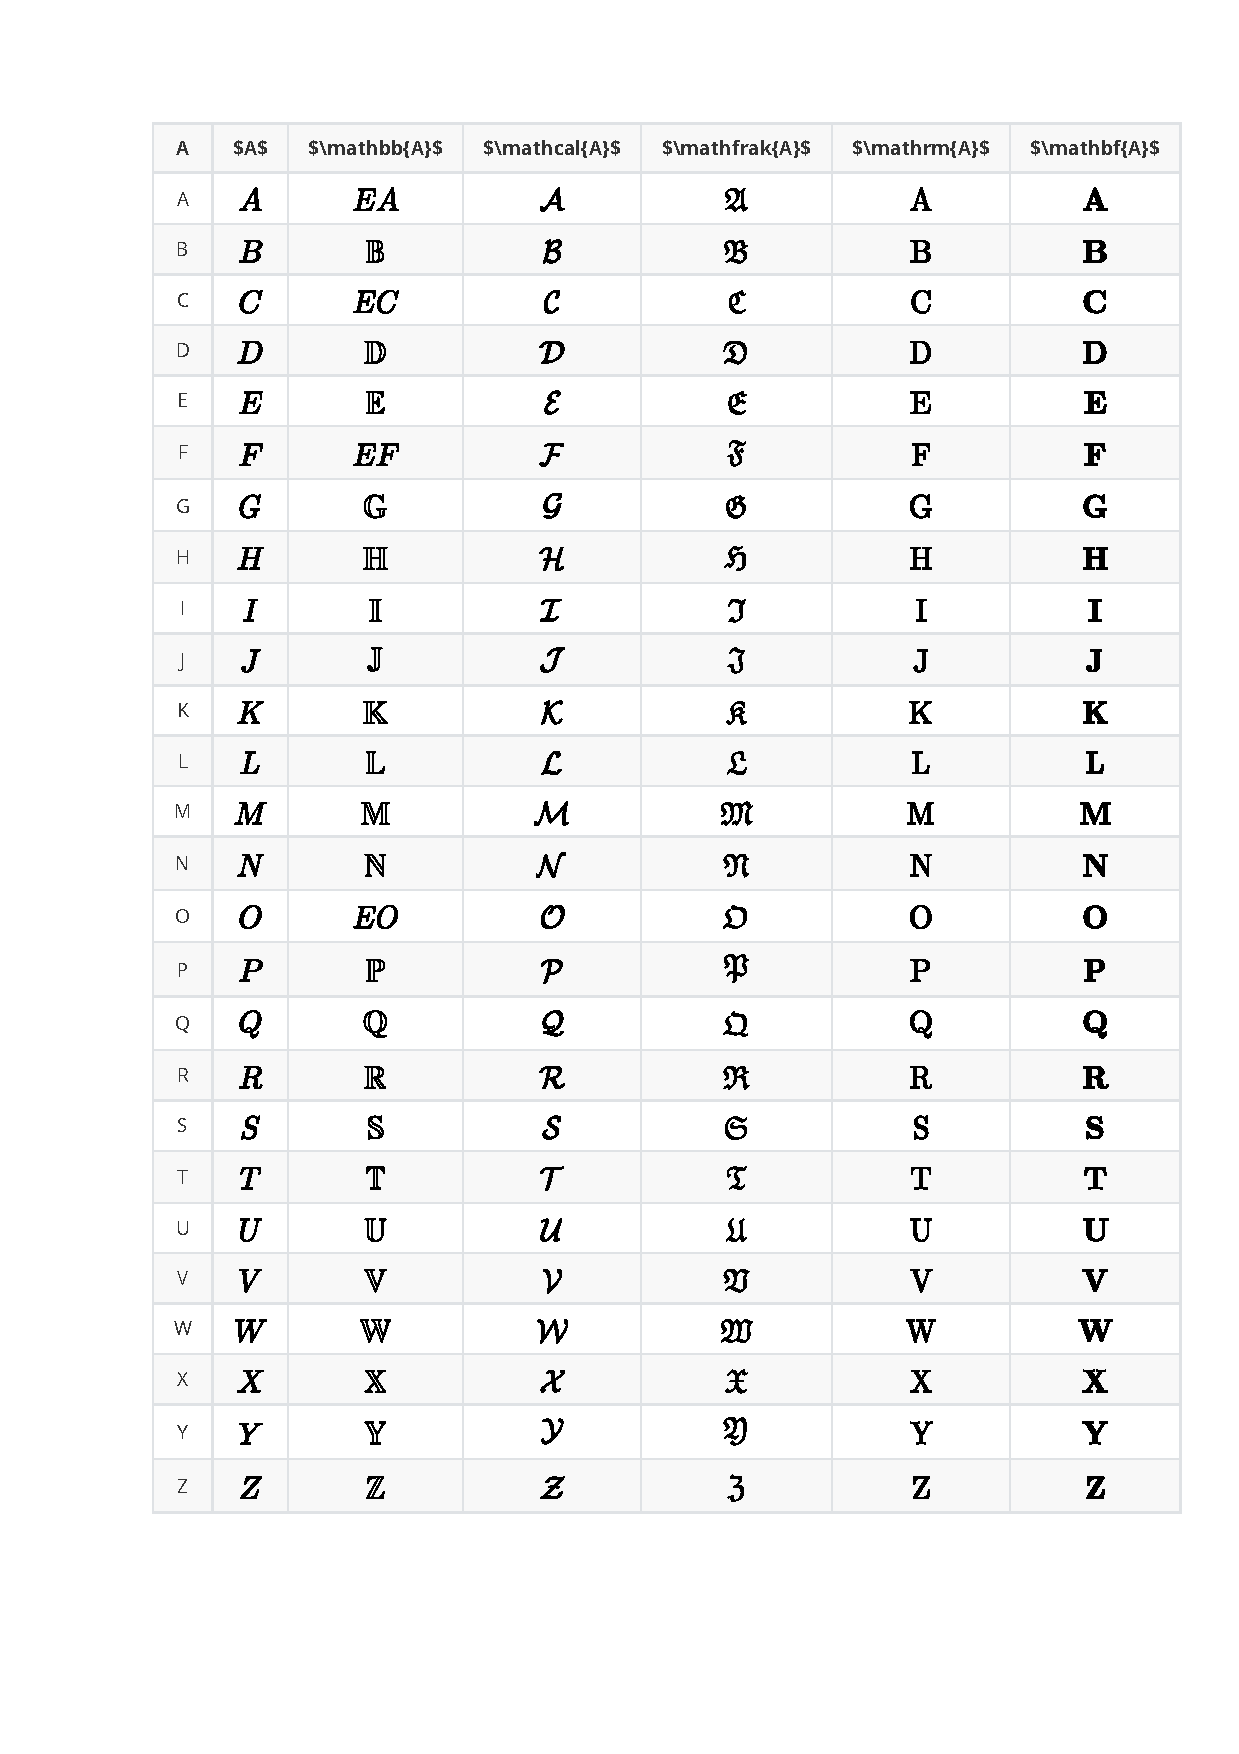
\includepdf{mathfonts.pdf}

\subsection{\LaTeX 中的颜色}
参考\href{http://latexcolor.com/}{latexcolor}。

\subsection{注脚}
两种常用形式:
\begin{itemize}
	\item \begin{verbatim}\footnote{注脚的内容}\end{verbatim}
	\item 这种方式很方便,可以在多处共享一个注脚,只需使用同一个注脚编号即可
	\begin{verbatim}
		\footnotemark[注脚编号]
		\footnotetext[编号]{注脚内容}
	\end{verbatim}
\end{itemize}

\subsection{章节编号}
默认是从1开始编号的,如果要从0开始,可以加一条命令:\begin{verbatim}\setcounter{section}{-1}\end{verbatim}


\subsection{常用符号}
\begin{myitemize}
	\item 约等于$\approx$ : \verb|\approx|
	\item $\approxeq$ : \verb|\approxeq|
\end{myitemize}






